% !TeX spellcheck = en_GB
% %%% ***************** CHAPTER INTRODUCTION ***************** %%%
\chapter{Introduction}
\label{ch:intro}
%%%%%%%%% INTRODUCTION %%%%%%%%%%%%%%
An increased frequency of extreme weather events and heat waves, droughts, heavy rains or extremely high winds is one predicted consequence of global warming \citep{hansen_warmer_2014}. Weather and climate extremes can have serious effects on human society and infrastructure, as well as on ecosystems and wildlife. Severe weather events are mostly in the focus of media reports on the topic of climate warming \citep{meehl_introduction_2000}. Understanding and predicting the impact of extreme weather events is one of the major challenges of current climate research \citep{stocker_working_2013,field_summary_2014}.
\par\medskip
\noindent
This work focuses on the extreme event during Christmas 2016, and the measurements and model forecasts taken at the measurement site Haukeliseter in Southern Norway. The extreme storm was named 'Urd' by the Norwegian Meteorological Institute (Met-Norway), and had a large impact on Norway. Storms of this kind are expected to occur on average every five years. The financial costs associated with 2016 Christmas storm are estimated to about 180 million Norwegian kroner. 'Urd' led to major traffic problems for cars, trains, ferries and air planes. Most mountain crossings were kept closed during Christmas 2016 \citep{olsen_ekstremvaerrapport._2017}. A change in temperature and therefore a change of frozen to liquid precipitation followed by an increase in avalanche danger. In addition, a power blackout of around 70.000 households where 40 emergency power stations failed during the extreme weather (\Cref{fig:news}). Since people are affected by extreme weather it is important to accurately measure and forecast severe storms. The use of accurate observations will lead to better performing weather forecast models, which rely heavily on observations \citep{joos_influence_2012}. 
%%% images from Twitter and news %%%%%%%%%%%%%%%%%%%%%%%%%%%%%%%%%%%%%
% !TeX spellcheck = en_GB
\begin{figure}[t!]
	\centering
	\begin{subfigure}[b]{0.49\textwidth}
		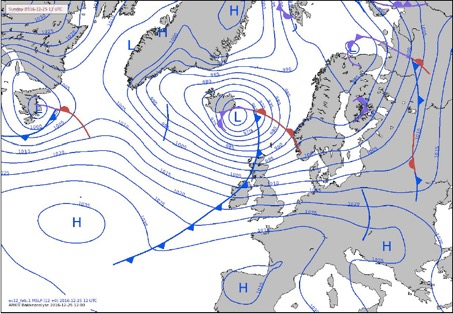
\includegraphics[width=\textwidth]{./fig_introduction/Ana_2512_12UTC.jpg}
		\caption{}\label{fig:ana_YR}
	\end{subfigure}
\hfill
	\begin{subfigure}[b]{0.49\textwidth}
		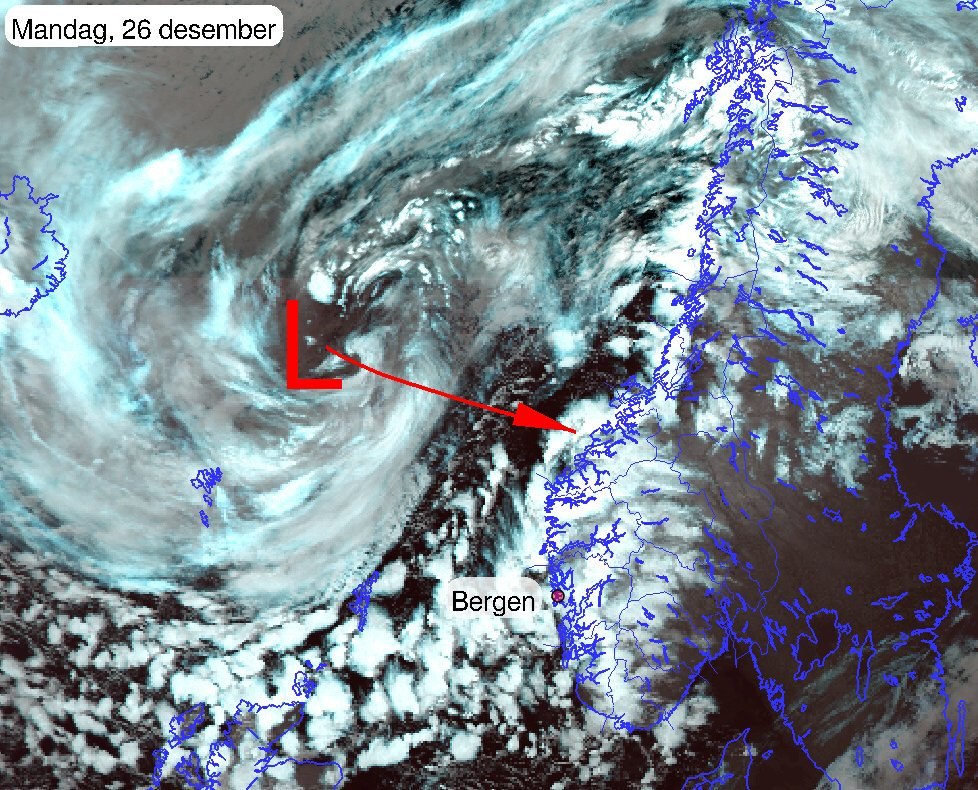
\includegraphics[trim={0cm 3.8cm 0cm 0cm},clip, width=\textwidth]{./fig_introduction/Twitter_26122016_0934AM.jpeg}
		\caption{}\label{fig:meteorologene_2612}	
	\end{subfigure}
	\begin{subfigure}[b]{0.49\textwidth}
		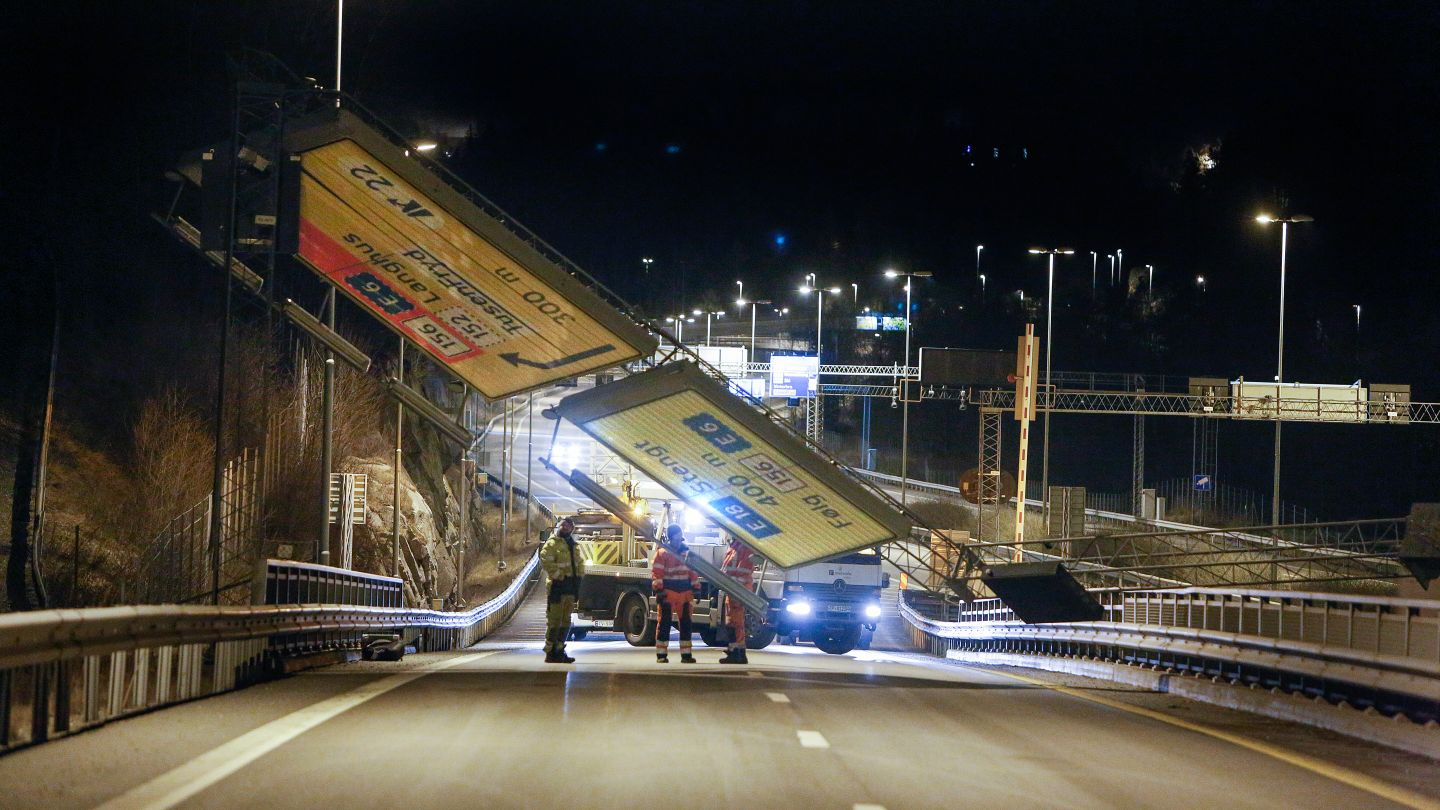
\includegraphics[width=\textwidth]{./fig_introduction/street_sign_2512.jpg}
		\caption{}\label{fig:street_sign}
	\end{subfigure}
\hfill
	\begin{subfigure}[b]{0.49\textwidth}
		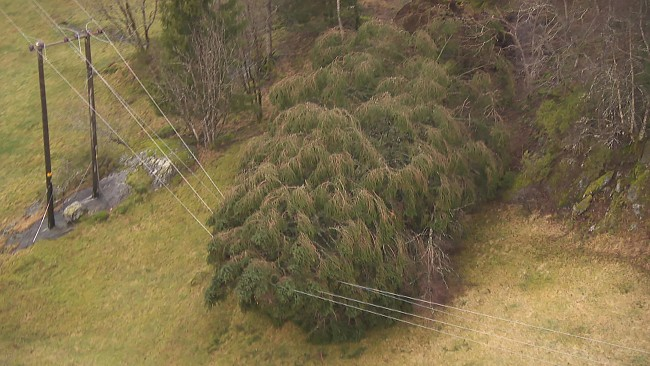
\includegraphics[width=\textwidth]{./fig_introduction/tree_nrk_2812.jpg}
		\caption{}\label{fig:tree_elec}
	\end{subfigure}
\caption{Weather situation during the extreme Christmas storm and impact on the infrastructure. In \protect\subref{fig:ana_YR}: Weather situation Sunday \SI{25}{\dec} at \SI{12}{\UTC} from the extreme weather report on Urd \citep{olsen_ekstremvaerrapport._2017}.
	\protect\subref{fig:meteorologene_2612}: Tweet from \cite{meteorologene_her_2016} on \SI{26}{\dec} at 9:34 am: Here comes \#Urd! The low pressure centre will hit M{\o}re og Romsdal, but the strongest wind comes south of Stad. \#S{\o}rNorge.
    \protect\subref{fig:street_sign} and \protect\subref{fig:tree_elec} show the consequences related to the high wind speeds during Christmas 2016.
	\protect\subref{fig:street_sign}: This traffic sign, ten meter long and four meter high was blown down during the storm, \citep{ruud_tonn_2016}.
	\protect\subref{fig:tree_elec}: Trouble maker: The extreme weather during Christmas created problems for the local infrastructure. \num{80.000} households were without electricity during the storm, \citep{farestveit_80.000_2016}.} \label{fig:news}
\end{figure}
%%%%%%%%%%%%%%%%%%%%%%%%%%%%%%%%%%%%%%%%%%%%%%%%%%%%%%%%%%%%%%%%%%%%%%%%%%
\par\medskip
\noindent
Since winter 2010, Haukeliseter has been a WMO measuring station with single and double fence precipitation instruments. In the winter of 2016/2017, three additional state of the art radar and snowflake microphysical instruments were deployed, which could be used to estimate the vertical profile of snow water content in the atmosphere. \citet{joos_influence_2012} showed that when sensitivity studies on a regional model is applied, the storm development depends on whether or not the placement of the precipitation is correct in the simulated storm. Looking at the vertical precipiation, which determines the vertical profile of latent heating, and hence leading to potential vorticity generation or destruction which then in turn will lead to a storm amplification or decrease, respectively. Vertical pointing radar reflectivities are rare but can be an improvement to understand the microphysical structure in storms. Therefore, radar reflectivities were measured using the \SI{24}{\giga\hertz} Micro Rain Radar (MRR) at Haukeliseter. Snowflake characteristics were estimated using a Multi-Angle Snowflake Camera \citep[MASC;][]{garrett_fall_2012} and a Precipitation Imaging Package \citep[PIP;][]{newman_presenting_2009}. 
%With the aid of the modified CloudSat snow particle model algorithm and the snowflake properties, as well as reflectivity profiles, the amount of snowfall in the atmosphere can then be determined. 
An optimal-estimation retrieval algorithm was developed that could estimate  snowfall rates consistent with each MRR, MASC, and PIP measurement.  
The double fence measurements %should help to estimate vertically derived snowfall on the ground.
will provide a boundary condition to ensure that retrieved surface snowfall accumulations are close to the truth. Such agreement will in turn provide confidence that retrieved snow water contents in the vertical are also valid.
\\
The Meteorological Cooperation on Operational Numerical Weather Prediction (MetCoOp) Ensemble Prediction forecast (MEPS) has been operational at Met-Norway, since 2016. The ensemble prediction system uses the previous deterministic AROME-MetCoOp, a version of the Mèteo-France Applications of Research to Operations at Mesoscale. In addition, ten perturbed ensemble members are initialised in MEPS. The newly developed ensemble prediction systems (EPS) from Met-Norway is used to analyse the extreme winter storm during Christmas 2016. It will be shown in the thesis if the ensemble prediction system is able to forecast the variation of an extreme winter event such as 'Urd' and if the forecast model is able to predict large scale as well as local effects. Furthermore, the use of an ensemble prediction system will give the possibility to compare the variation of snowfall precipitation at the surface and in the vertical. Observations will help to compare MEPS model forecast to examine the following research questions: 
How well will the model predict the surface snowfall at the measurement site? Will large scale phenomena be predicted by MEPS?
Does the regional model cover local affects associated with the topography around the site?
%%%%%%%%%%%%%%%%%%%%%%%%%%%%%%%%%%%%%%%%%%%%%%%%%%%%%%%%%%%%	


\section{Background}
It has long been known that measuring precipitation, especially in the form of snow, is difficult. Winter precipitation measurement show biases of more than \SI{100}{\percent} between different gauge observation networks and different regions \citep{kochendorfer_analysis_2017}. The local climate changes from station to station leading to different habit and size of frozen aggregates. Measurement uncertainties can be caused by the instrument itself, which varies with wind speed, gauge wind shielding, shape, size, phase, and fall velocity in hydrometeors \citep{kochendorfer_analysis_2017,wolff_derivation_2015}. 
Uncertainties in precipitation measurements under windy conditions can affect water balance calculation and the calibration of remote sensing algorithms \citep{wolff_derivation_2015}. 
\\
Precipitation observations are important for hydrological, climate and weather research, as more than one-sixth of the world's population receives water from glaciers and seasonal snow packs \citep{barnett_potential_2005}.
\\
Since winds have an influence on frozen precipitation, a WMO (World Meteorological Organization) precipitation analysis between 1987 and 1993 recommended, that the double-fence inter-comparison reference should be used as a reference for snow measurements \citep{goodison_wmo_1998}. An adjustment for unshielded and single-shielded precipitation gauges followed in 2010. The adjustment transfer function, for single fence gauges, represents a capture efficiency as a function of air temperature and wind speed to delimit the error of measured snowfall \citep{kochendorfer_analysis_2017,wolff_derivation_2015}.
\par\medskip
\noindent
Estimates of snowfall from radar reflectivities are non-unique. 
%Nearly identical snowfall rates for given radar reflectivity signatures can be generated from various combinations of snowflake microphysical properties and particle fall velocity.
This means, a given reflectivity can yield very different estimates of snowfall depending upon the precise microphysical assumptions used in the retrieval scheme.
%This can lead for individual events to an error in retrieval uncertainties of \num{100}--\SI{200}{\percent} \citep{wood_estimation_2011}. 
\citet{kulie_utilizing_2009}, for example, used the CloudSat Cloud Profiling Radar (CPR) reflectivities to estimate the global precipitation rate of dry snowfall through one year. They found that snowfall estimates critically depend on assumed snowfall particle size distribution, shape, and radar reflection. 
%These studies suggest that snowfall estimates resulting only from radar reflections are ambiguous. Numerous different combinations of snowflake microphysical properties and snow particle falling rates can yield to nearly identical surface snowfall rates for a given reflectivity profile. 
They concluded, that the use of traditional Ze-S relationships can lead to large differences when comparing snowfall events with different microphysics.
\\
%Based on observations of particle size distribution, fall velocity, snowflake habit, and a modified version of the optimal estimation CloudSat snowfall algorithm followed an average difference reduction to \SI{18}{\percent} of snowfall estimates, when compared to a National Weather Service measurement in Barrow, Alaska \citep{cooper_variational_2017}.
Subsequent studies have tried to incorporate scene dependent microphysical information into the retrieval scheme.  \citet{wood_estimation_2011} embedded particle size distribution (PSD) - temperature relationship information into the CloudSat operational snowfall retrieval scheme to help reduce retrieval non-uniqueness. \citet{cooper_variational_2017} used in-situ estimates of snowflake PSD and habit from ground-based instrumentation to explore snowfall retrieval performance at Barrow, Alaska. They found reasonable agreement within \SI{20}{\percent} of nearby snow gauge measurements.
\par\medskip
\noindent
With the increasing expansion of computational power, developments of high-resolution numerical weather forecasting models with $\le$\SI{4}{\km} scales can be able to represent small-scale phenomena, such as convective dynamics \citep{gowan_validation_2018}. This enhancement provides weather services the ability to improve short-term weather forecasts for convective events, which can seriously impact infrastructure and society \citep{muller_arome-metcoop:_2017}. 
Information on magnitudes and location of maximum temperature is of significant importance when warnings are published by meteorologcial services for severe weather events and for further use in downstream impact model, e.g. NVE's (Norwegian Water Resources and Energy Directorate) hydrological model for flooding and avalanche risk.
The ability to use high-resolution models is also followed by various challenges, such as physical parametrisation schemes, accurate representation of topography, and data assimilation of high-resolution data \citep{sun_convective-scale_2005}.
\\
The weather forecast in Scandinavia covers a wide range of phenomena and includes continental, maritime and polar conditions. Norway has a complicate coastline, gradients in land use, as well as complex topography, which can complicate local weather forecasting of temperature, wind and precipitation \citep{muller_arome-metcoop:_2017}. \citet{colle_1314_2005,garvert_1314_2005,schwartz_reproducing_2014}, for example, have shown, that simulations of orographic precipitation can be improved in mountainous terrain for horizontal grid spacing below \SI{4}{\km}. Uncertainties on a convective scale can lead to a rapid error growth \citep{lorenz_atmospheric_1969}, hence high-resolution ensemble prediction makes it possible to estimate the forecast uncertainty by performing several model runs, each with different initial conditions. %\citep{gowan_validation_2018}
\par\medskip
\noindent
The Christmas storm in 2016, might not have led to the same damages as some of the extreme weather events of recent years. As people and infrastructure are affected by extreme weather, it is necessary to further improve the accuracy of snow-ground observations to better verify numerical weather forecasts, hydrological and climate models \citep{joos_influence_2012}. Changes in snow pack characteristics after extreme rain on snow events can lead to severe avalanches \citep{stimberis_glide_2011} and to the formation of thick layers of ice in the snow pack or on ground \citep{putkonen_rain--snow_2003,hansen_climate_2011}.
%%%%%%%%%%%%%%%%%%%%%%%%%%%%%%%%%%%%%%%%%%%%%%%%%%%%%%%%%%%%

\section{Descripition of this study}
The purpose of this study is to apply an optimal-estimation snowfall retrieval on ground based measurements to estimate the surface accumulation and vertical snow water content for an extreme event during Christmas 2016. These will later be used to compare to \SI{48}{\hour} MEPS model forecasts to see if the model was able to predict synoptical features and precipitation related to the extreme event 'Urd' in 2016. 
\par\medskip
\noindent
This method of estimating snowfall is much like the study from \citet{cooper_variational_2017}. The main difference between the studies at Barrow, Alaska and this study is that a \SI{24}{\giga\hertz} MRR is used instead of a \SI{94}{\giga\hertz} Ka-band ARM zenith radar, and PSD and fall speed is estimated from MASC, PIP images and Doppler velocities, respectively.
\\
The comparison of the surface MEPS forecasts is similar to \citet{muller_arome-metcoop:_2017}. They presented the performance of the previous operational model at Met-Norway, AROME-MetCoOp, to the global forecast system ECMWF. Case studies were provided to demonstrate the ability of the deterministic model to capture extreme precipitation and wind events. 
\par\medskip
\noindent
The thesis is structured as following: \Cref{ch:Methods} will give an overview of the measurement site Haukeliseter and its instrumentation, followed by the methodology on the optimal estimation retrieval as well a description of the regional model MEPS. The application to the data will be presented to compare the forecast system to the observations. The synoptics of the extreme Christmas storm in 2016 is analysed in \Cref{ch:weather_ana}. \Cref{ch:Res} will show the results and the discussion on large scale effects, surface snowfall accumulation and local wind influence  at Haukeliseter. The final chapter summarises the results and findings and suggests future research questions.